\chapter{Graph Exploration and Structural Insights}
\label{chap:graph_exploration}

\section{Why Explore the Graph Before Prediction?}

It is tempting to treat the graph built in Chapter~\ref{chap:kg} as a
black box that is fed into a GNN and evaluated by a single F1 number.
That view is wrong for two reasons.

First, \emph{the graph is the dataset}. In a flat-text pipeline the
dataset is a set of labelled documents; here the dataset is a typed,
relational object with cross-domain structure, and any claim a later
chapter makes about the model's behaviour presupposes a concrete
understanding of that structure. Whether the model's accuracy is
driven by genuine cross-case reasoning or by a few dominant hub
statutes, whether the five legal domains are actually five or mostly
one, whether the per-case subgraph has the connectivity a
message-passing layer needs -- none of these questions can be answered
by looking at prediction results alone.

Second, \emph{leakage-safety claims are structural claims}. The
leakage prevention strategy in
Section~\ref{sec:leakage_prevention} is only as convincing as the
structural evidence that the remaining graph is still dense enough to
support learning. If removing RPC annotations, decision fields, and
identity-proxy shortcuts left behind a near-disconnected graph, the
downstream accuracy would be either implausibly high (still leaking)
or implausibly low (now uninformative). The exploration stage is
where we verify that neither is the case.

This chapter therefore treats the graph as an object of study in its
own right. Section~\ref{sec:graph_stats} summarises the overall
structure; Section~\ref{sec:perdomain} breaks it down per legal
domain; Section~\ref{sec:key_insights} distils the conclusions that
feed forward into Chapter~\ref{chap:results}.

\section{Graph Statistics and Structural Analysis}
\label{sec:graph_stats}

\subsection{Overall Graph Statistics}

The final reasoning-focused graph, assembled across all five legal
domain buckets, contains \textbf{880{,}176 nodes} and
\textbf{1{,}977{,}295 edges}. The average node degree is
\textbf{4.49}; the maximum degree is \textbf{29{,}602}, attained by
the \textsc{IPC} statute node.

At the per-bucket level (before cross-bucket sharing is expanded into
the unified view the GNN trains on), the five buckets have broadly
comparable case counts but markedly different internal densities:

\begin{table}[H]
  \centering
  \small
  \begin{adjustbox}{max width=\textwidth}
  \begin{tabular}{lrrr}
    \toprule
    Bucket & Cases (files) & Nodes & Edges \\
    \midrule
    Family \& Matrimonial & 15{,}307 & 97{,}150 & 3{,}660{,}068 \\
    Financial Fraud & 14{,}616 & 113{,}240 & 7{,}869{,}952 \\
    Land \& Property & 14{,}052 & 126{,}962 & 9{,}210{,}612 \\
    Motor Accidents & 15{,}237 & 125{,}234 & 7{,}165{,}461 \\
    Sexual Offences & 14{,}597 & 106{,}662 & 7{,}123{,}225 \\
    \midrule
    \textbf{Cross-bucket unified} & \textbf{73{,}809} & \textbf{485{,}540}
      & \textbf{27{,}243{,}141} \\
    \bottomrule
  \end{tabular}
  \end{adjustbox}
  \caption{Per-bucket and cross-bucket graph statistics. The
  cross-bucket graph is denser than the sum of the per-bucket graphs
  because shared \textsc{Statute}, \textsc{Provision}, and
  \textsc{Precedent} nodes acquire edges from every bucket that cites
  them.}
  \label{tab:graph_stats}
\end{table}

Family-matrimonial is the sparsest bucket by edges-per-case
(\(\approx 239\)), and land-property is the densest (\(\approx 655\));
the difference is driven mostly by the number of distinct provisions
and precedents cited per case in each domain.

\subsection{Node Type Distribution}

The node-type breakdown of the unified graph is strongly skewed
towards \textbf{parties and precedents}:

\begin{table}[H]
  \centering
  \small
  \begin{adjustbox}{max width=\textwidth}
  \begin{tabular}{lrr}
    \toprule
    Node type & Count & Share \\
    \midrule
    \textsc{Case}        &  72{,}735 &  8.3\% \\
    \textsc{Precedent}   & 255{,}148 & 29.0\% \\
    \textsc{Respondent}  & 192{,}147 & 21.8\% \\
    \textsc{Petitioner}  & 171{,}084 & 19.4\% \\
    \textsc{Lawyer}      &  73{,}645 &  8.4\% \\
    \textsc{Provision}   &  43{,}504 &  4.9\% \\
    \textsc{Court}       &  38{,}799 &  4.4\% \\
    \textsc{Statute}     &  21{,}754 &  2.5\% \\
    \textsc{Judge}       &  11{,}360 &  1.3\% \\
    \bottomrule
  \end{tabular}
  \end{adjustbox}
  \caption{Distribution of the 880{,}176 nodes by type in the unified
  reasoning-focused graph.}
  \label{tab:node_type_dist}
\end{table}

Understanding which of these node types are \emph{shared} across cases versus
\emph{local} to a single case is central to understanding how information can
propagate through the graph. Shared nodes are the mechanism by which a GNN can
transfer knowledge from one case to another; local nodes contribute features
only to the case they belong to. Figure~\ref{fig:shared_vs_local} visualises
this split per bucket.

\begin{figure}[H]
  \centering
  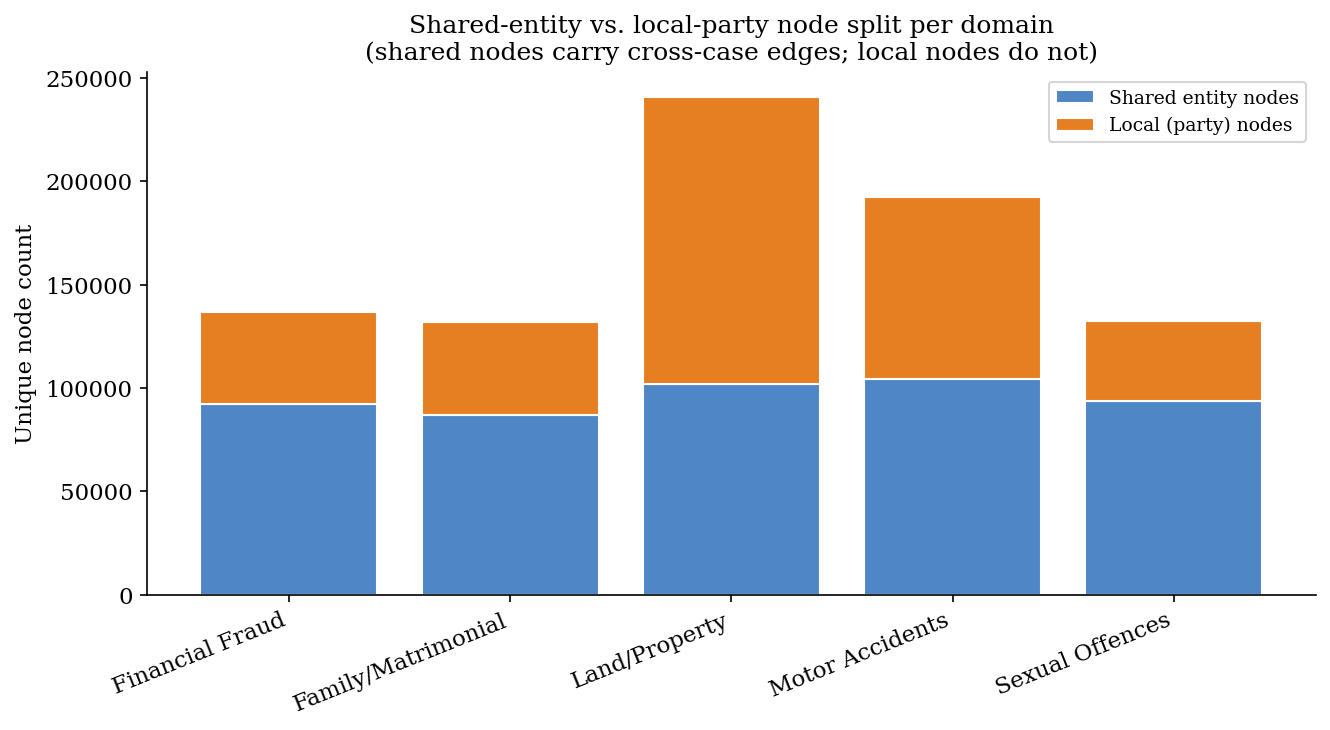
\includegraphics[width=0.92\textwidth]{figures/41_shared_vs_local_nodes_per_bucket.png}
  \caption{Shared versus local node counts per legal domain bucket. Party nodes
  (\textsc{Petitioner}, \textsc{Respondent}, most \textsc{Lawyer} nodes) are
  almost entirely local --- a party in one case rarely recurs in another.
  Statutes, provisions, courts, and frequently-cited precedents form the shared
  layer that is the graph's cross-case connective tissue.}
  \label{fig:shared_vs_local}
\end{figure}

The figure confirms that the split is sharp and legally interpretable. Party nodes
are almost entirely local: a petitioner or respondent in one matter rarely appears
in another unrelated case. Statutes, provisions, courts, and frequently-cited
precedents, by contrast, form a small but densely shared layer. This is the layer
through which all cross-case message passing must flow. The implication is that
removing party nodes from the shared layer---as the leakage-safe design does for
judges and specific lawyers---does not destroy cross-case connectivity; the
statute and precedent layer remains fully intact and is the genuine information
carrier. The statute side of the graph is small in node count but, as the next
subsection shows, carries disproportionate structural weight.

\subsection{Degree Distribution and Hub Entities}

The graph is strongly hub-dominated. The top-12 nodes by degree are
all statutes, provisions, or courts -- exactly the node types the
schema shares across cases:

\begin{table}[H]
  \centering
  \small
  \begin{adjustbox}{max width=\textwidth}
  \begin{tabular}{llrr}
    \toprule
    Node & Type & Degree & Buckets bridged \\
    \midrule
    IPC                                   & Statute   & 29{,}602 & 5 \\
    CR.P.C.                               & Statute   & 18{,}704 & 5 \\
    Supreme Court                         & Court     & 17{,}294 & 5 \\
    Apex Court                            & Court     & 14{,}242 & 5 \\
    Indian Penal Code                     & Statute   & 12{,}009 & 5 \\
    High Court of Judicature at Allahabad & Court     &  8{,}833 & 5 \\
    Section 482                           & Provision &  8{,}732 & 5 \\
    Section 506                           & Provision &  8{,}258 & 5 \\
    I.P.C.                                & Statute   &  7{,}051 & 5 \\
    Section 420                           & Provision &  6{,}285 & 5 \\
    Section 323                           & Provision &  6{,}002 & 5 \\
    Constitution of India                 & Statute   &  5{,}950 & 5 \\
    \bottomrule
  \end{tabular}
  \end{adjustbox}
  \caption{Top hub entities by degree, with the number of buckets they
  bridge. Every one of the top 12 hubs appears in all five legal
  domains.}
  \label{tab:top_hubs}
\end{table}

The PageRank ranking tells the same story from a different angle:
IPC ($\text{PR}=0.0114$), Supreme Court ($0.0082$), CR.P.C.\
($0.0069$), and Apex Court ($0.0067$) dominate the top of the
distribution. That every one of the top hubs bridges all five buckets
is not an accident of the numbers -- these are the statutes and
courts every Indian criminal and civil proceeding touches -- but it
has a concrete modelling consequence: these hubs are where cross-case
message passing actually happens.

To understand whether this hub dominance is a localised anomaly or a systemic
structural feature, Figure~\ref{fig:degree_ccdf} plots the complementary
cumulative degree distribution (CCDF) on a log-log scale.

\begin{figure}[H]
  \centering
  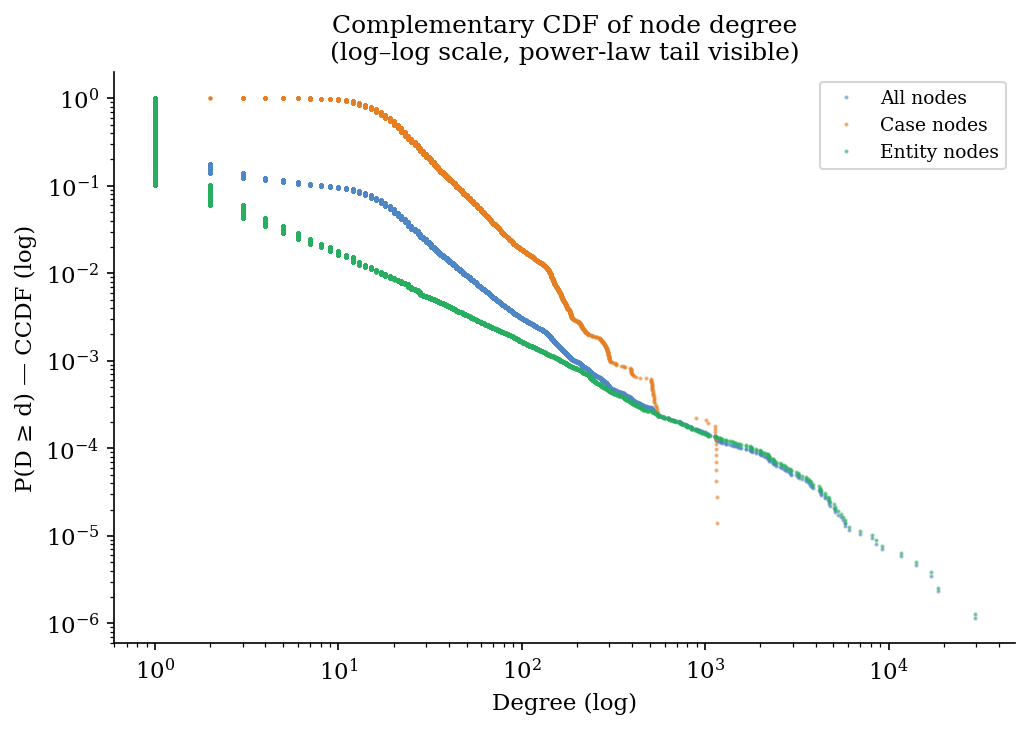
\includegraphics[width=0.92\textwidth]{figures/37_degree_ccdf_loglog.png}
  \caption{Complementary cumulative degree distribution (CCDF) of the unified
  graph on a log-log scale. The approximately linear decay is the hallmark of a
  heavy-tailed degree distribution: most nodes have very low degree, while a
  small number of hub nodes accumulate orders of magnitude more edges than the
  average, confirming that hub dominance is a systemic structural feature rather
  than an artefact of a few outliers.}
  \label{fig:degree_ccdf}
\end{figure}

The approximately linear decay in this plot is the signature of a heavy-tailed,
scale-free-like degree distribution. The vast majority of nodes sit at degree
one or two, while a thin upper tail extends to degrees of tens of thousands.
This two-regime structure -- a small set of super-hubs plus a long tail of
single-case leaves -- has a direct modelling consequence: message passing
aggregates over all neighbours, so hub nodes receive and broadcast information
from a disproportionately large fraction of the graph. The cross-case reasoning
capacity of the GNN is therefore structurally concentrated in a handful of
statute and court nodes. The ``connectivity score'' in
Section~\ref{sec:connectivity} is designed to quantify how well each individual
case is wired into this hub layer.

\subsection{Cross-Domain Bridge Analysis}

The buckets are not isolated. Table~\ref{tab:top_hubs} already shows
that the top hubs are bridges by construction; the full bridge
analysis confirms that the connective tissue between domains is
dominated by the general criminal-procedure and penal-code statutes,
with domain-specific bridges layered on top:

\begin{itemize}
  \item \textsc{IPC}, \textsc{CR.P.C.}, \textsc{Indian Penal Code},
    \textsc{Constitution of India}, and \textsc{Supreme Court} /
    \textsc{Apex Court} appear in all five buckets and together account
    for the majority of cross-bucket edges.
  \item Domain-specific statutes bridge fewer buckets but at higher
    within-bucket intensity: \textsc{POCSO Act} appears in four
    buckets but is heavily concentrated in sexual-offences;
    \textsc{Motor Vehicles Act, 1988} appears in all five but is
    concentrated in motor-accidents; \textsc{Land Acquisition Act,
    1894} is concentrated in land-property.
  \item Provisions like Section~482, 506, 420, and 323 are multi-bucket
    because they sit in the CrPC and IPC, which are themselves
    multi-domain.
\end{itemize}

To assess whether high degree and broad bridging are correlated or distinct
properties, Figure~\ref{fig:top_hubs_bridging} plots the top hub entities by
degree alongside the number of buckets they appear in, combining both dimensions
into a single view. The figure reveals that the two dimensions are correlated but
not identical: some high-degree nodes are concentrated within a single domain
(heavily-cited domain-specific provisions), while the universal bridges ---
\textsc{IPC}, \textsc{CR.P.C.}, \textsc{Supreme Court} --- sit at the top of
both rankings simultaneously. This distinction matters directly for cross-domain
transfer: only the universally shared hubs actually mediate information flow
between all five buckets during message passing. A high-degree domain-specific
hub, by contrast, influences prediction accuracy within its own bucket but
contributes nothing to cross-bucket generalisation.

\begin{figure}[H]
  \centering
  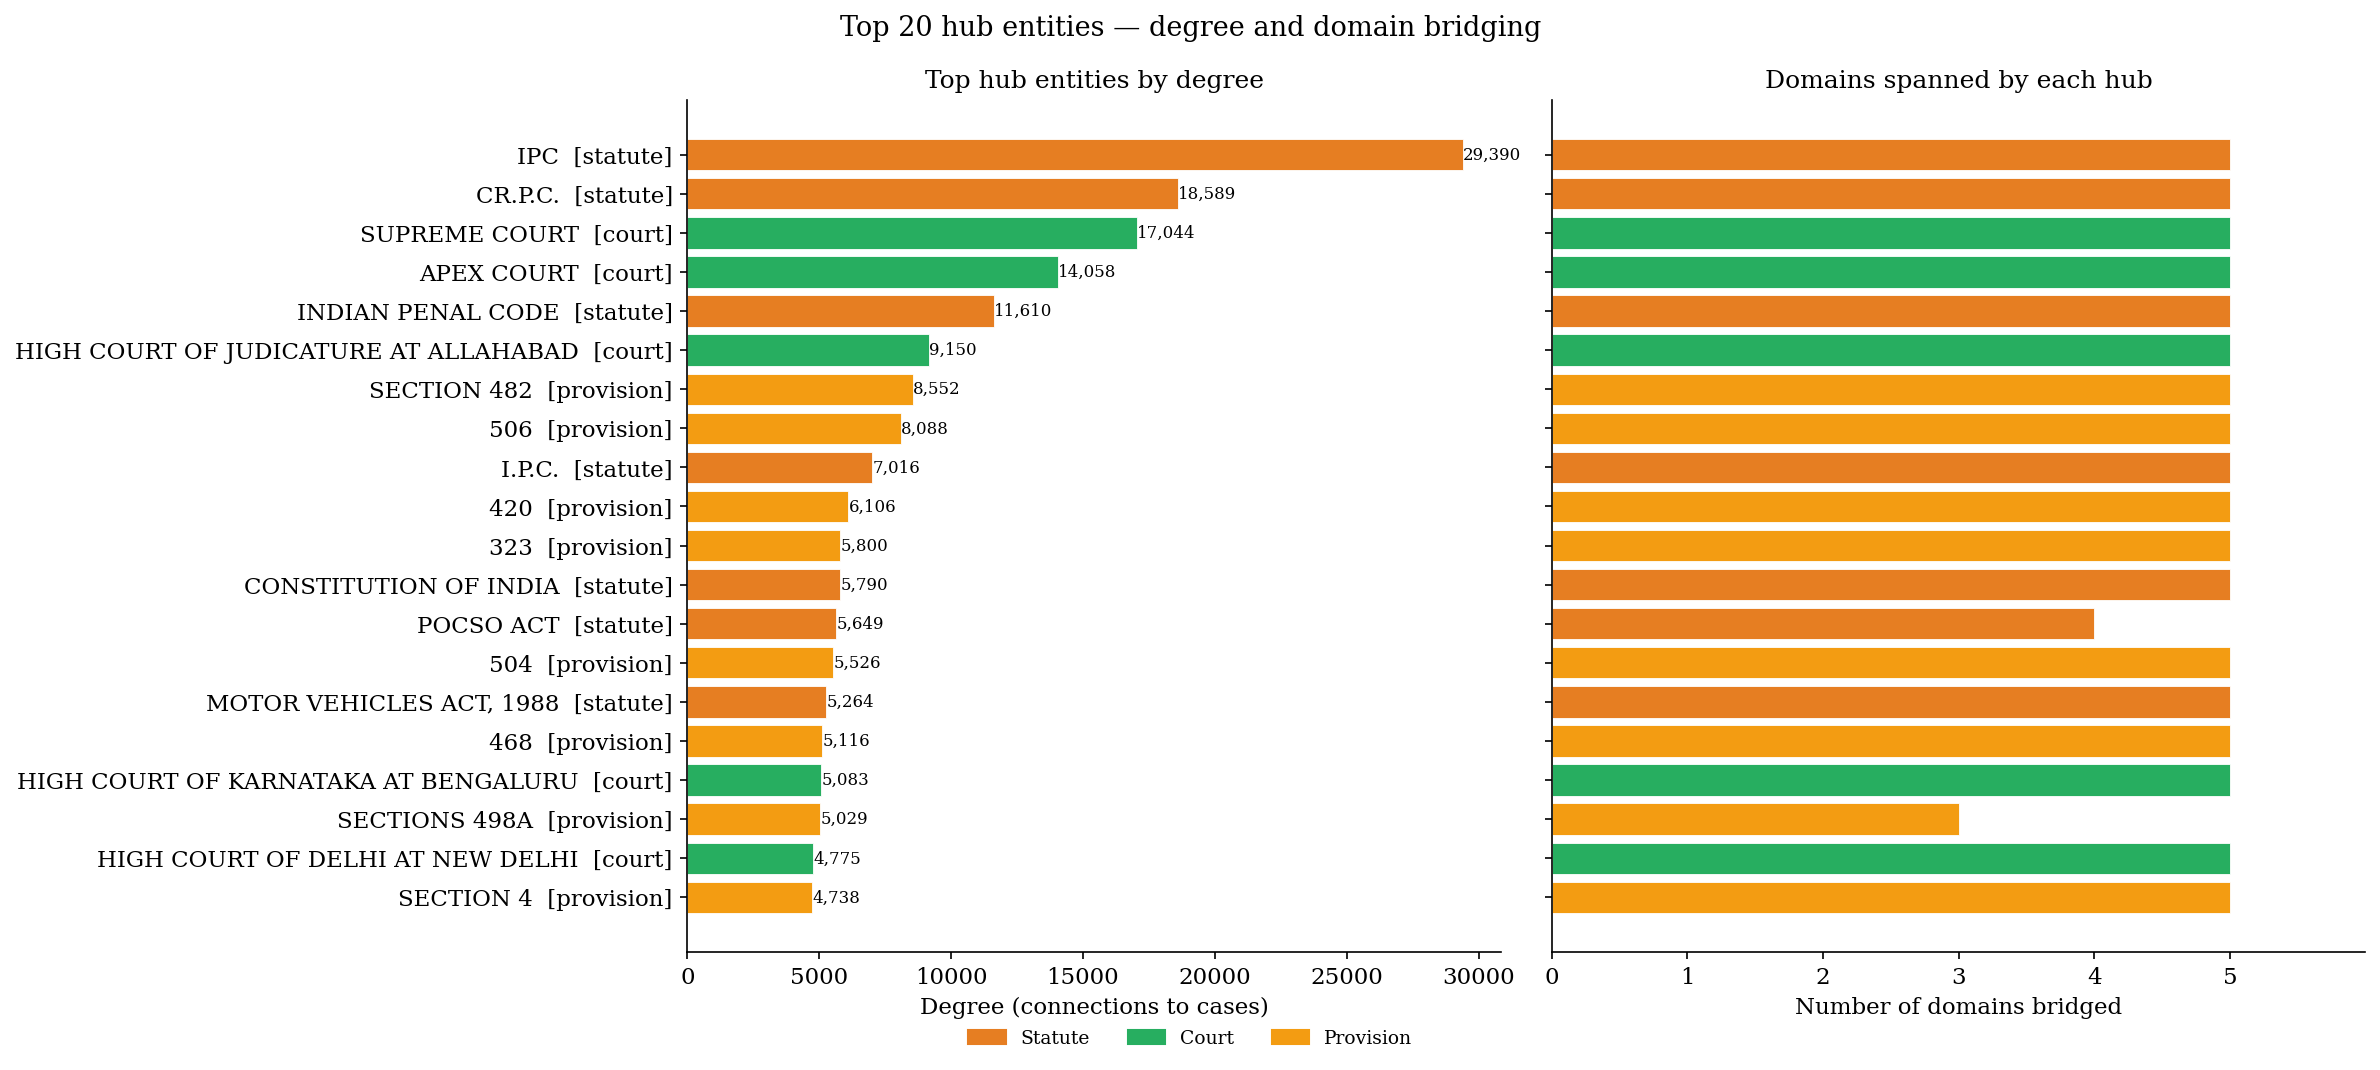
\includegraphics[width=0.92\textwidth]{figures/40_top_hubs_degree_and_bridging.png}
  \caption{Top hub entities ranked by degree, with the number of legal domain
  buckets they bridge encoded by colour or marker size. High degree and broad
  bridging are correlated but not equivalent: the universal bridges
  (\textsc{IPC}, \textsc{CR.P.C.}, \textsc{Supreme Court}) top both rankings,
  while domain-specific high-degree hubs appear in fewer buckets.}
  \label{fig:top_hubs_bridging}
\end{figure}

\subsection{Cross-Bucket Entity Sharing Matrix}

Knowing which individual nodes are hubs is useful; knowing how many entities
are shared \emph{between each pair of domains} is a different and complementary
question. If two domains share very few entities, cross-domain transfer between
them is structurally impossible --- there are no shared nodes for message passing
to flow through. If two domains share nearly all entities, they are functionally
the same graph and a separate bucket structure adds no value. The cross-bucket
sharing matrix in Figure~\ref{fig:cross_bucket_sharing_matrix} quantifies this
pairwise sharing at the canonicalised entity level across the full graph.

\begin{figure}[H]
  \centering
  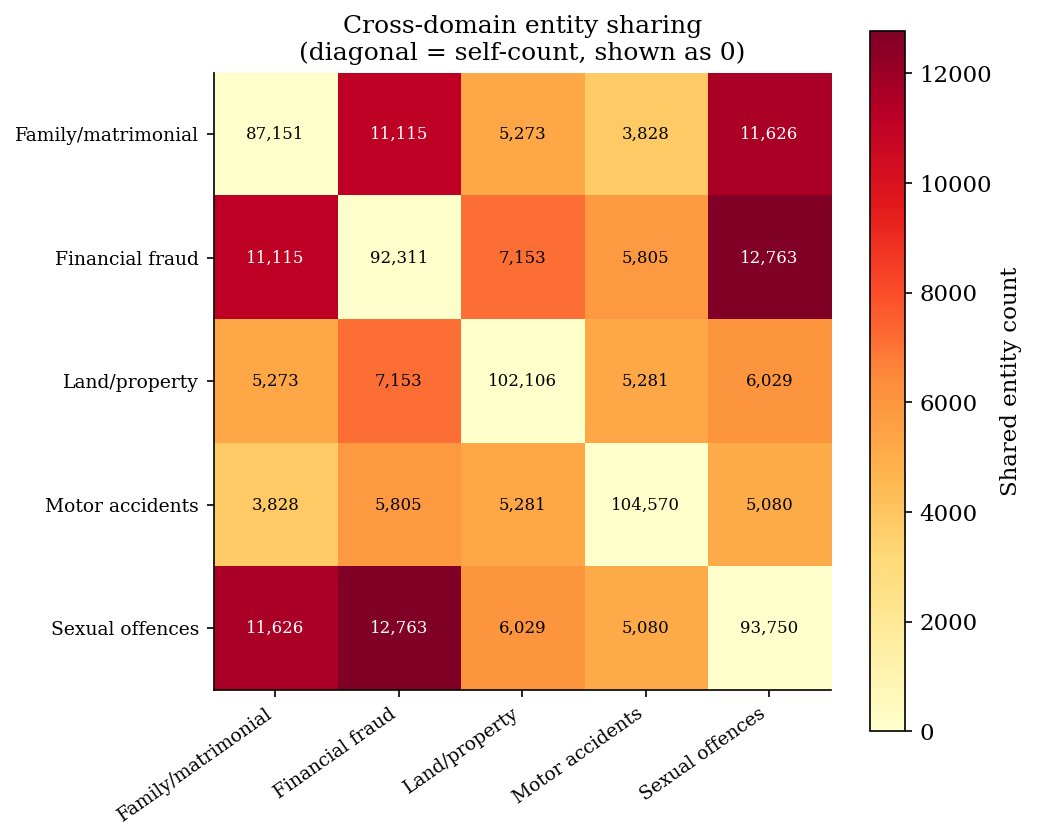
\includegraphics[width=0.9\textwidth]{figures/20_cross_bucket_sharing_matrix.png}
  \caption{Cross-bucket entity sharing matrix for the full graph. Each cell
  shows the number of canonicalised entities shared between two legal domain
  buckets. Darker values indicate more sharing. The three IPC/CrPC-driven
  buckets --- family-matrimonial, financial-fraud, and sexual-offences --- share
  heavily with each other; land-property is more weakly connected to the rest
  via its distinct statutory backbone.}
  \label{fig:cross_bucket_sharing_matrix}
\end{figure}

Three patterns are visible in the matrix:

\begin{enumerate}
  \item Strong pairwise sharing among \emph{Family \& Matrimonial},
    \emph{Financial Fraud}, and \emph{Sexual Offences} --- all three are
    IPC/CrPC-driven and share the same high-degree statute and provision nodes.
  \item Moderate sharing between those three and \emph{Motor Accidents},
    mediated by the general procedural statutes and by the Supreme Court and High
    Court nodes that every appellate domain shares.
  \item Comparatively weaker sharing with \emph{Land \& Property}, which is
    anchored by its own statutory backbone (Land Acquisition Act~1894,
    Constitution of India) and consequently has fewer canonical entities in
    common with the criminal-procedure-dominated domains.
\end{enumerate}

This pattern is exactly what a cross-domain transfer claim needs to be credible.
The domains are related enough that a shared graph representation should carry
useful signal across all five buckets; they are different enough that each bucket
retains its own statutory fingerprint and that a single-domain classifier should
not trivially dominate a cross-domain one. The moderate but not extreme sharing
level motivates the design choice of a unified cross-bucket graph rather than
five separate per-domain graphs: there is sufficient shared structure to benefit
from joint training, but sufficient domain separation to make that benefit
non-trivial.

\subsection{Connectivity Score Distribution}
\label{sec:connectivity}

The hub analysis above characterises individual nodes; a complementary question
is how well each \emph{case} as a whole is wired into the shared-entity layer.
A case that cites hub statutes and widely-cited precedents has many high-degree
shared neighbours and can therefore receive rich aggregated information from a
large neighbourhood during message passing. A case that sits primarily on rare
or single-occurrence entities is structurally isolated and receives little
cross-case signal. To make this distinction concrete, a \textbf{connectivity
score} is assigned to each case as a bucket-normalised measure of how well it
is connected to the rest of the graph through its shared-entity neighbours
(statutes, provisions, precedents). This score is important both as a
structural diagnostic and as a predictor of per-case modelling difficulty: a
GNN layer's information gain on a low-connectivity case is, by construction,
structurally bounded.

Figure~\ref{fig:connectivity_violin} shows the per-bucket connectivity score
distribution as a violin plot, which reveals not just the central tendency but
the full distributional shape.

\begin{figure}[H]
  \centering
  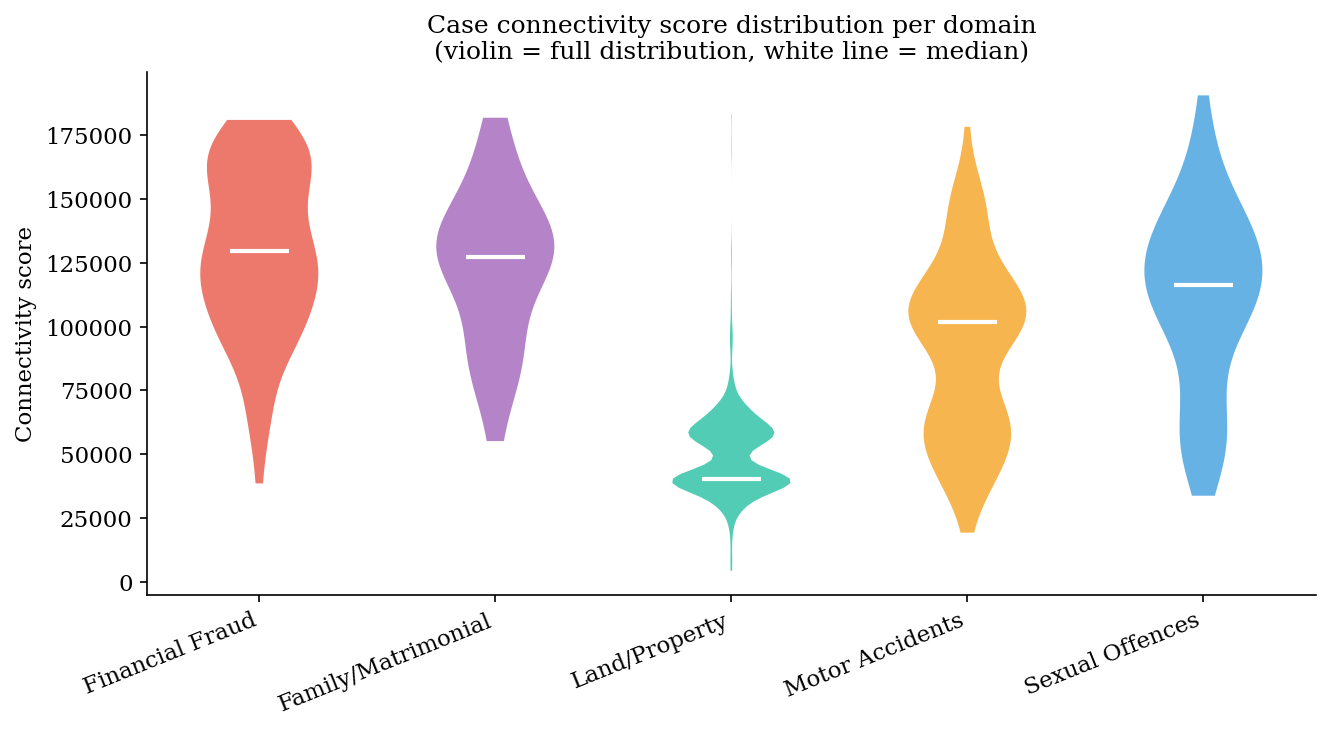
\includegraphics[width=0.9\textwidth]{figures/39_connectivity_violin.png}
  \caption{Per-bucket connectivity score distribution as violin plots. Land-property
  and financial-fraud show wider distributions with higher medians --- their cases
  cite more diverse authorities and are better connected to the graph's shared
  layer. Motor-accidents is sharply concentrated at low connectivity values,
  reflecting repeated citation of the same narrow provision set. Within-bucket
  variance predicts case-level prediction difficulty.}
  \label{fig:connectivity_violin}
\end{figure}

Land-property and financial-fraud show wider, higher-median distributions: their
cases cite diverse authorities and are therefore well-connected to the hub layer.
Motor-accidents shows a narrow distribution concentrated at low values, reflecting
the domain's repeated citation of the same small provision set (\textsc{Motor
Vehicles Act}, Section~166). The within-bucket variance is itself informative:
even within a single domain, cases span a substantial connectivity range, meaning
that prediction difficulty is heterogeneous at the case level and cannot be
attributed to domain alone. The ablation pattern in Chapter~\ref{chap:results}
is consistent with this expectation: cases in the low-connectivity tail of any
bucket show systematically higher error rates. The connectivity score is also
used by the Graph Visualiser (\path{GRAPH_VISUALISER/}) to rank cases when
sampling Hub-Network and Case-Connection views.

\section{Per-Domain Corpus Analysis}
\label{sec:perdomain}

The structural view above aggregates across buckets; the per-domain
view is where the legal character of each bucket shows up.

\subsection{Case Length and Sentence Distributions}

Case length varies substantially across buckets, and that variance is not merely
a descriptive curiosity --- it directly determines how text features are
constructed for the GNN. Long documents require chunked embedding strategies;
short documents can be embedded whole. Understanding the distribution shapes
the chunking configuration and lets us flag which domains will produce the most
embedding approximation.

Figure~\ref{fig:sentence_count_dist} shows the sentence-count distribution per
bucket across the full corpus.

\begin{figure}[H]
  \centering
  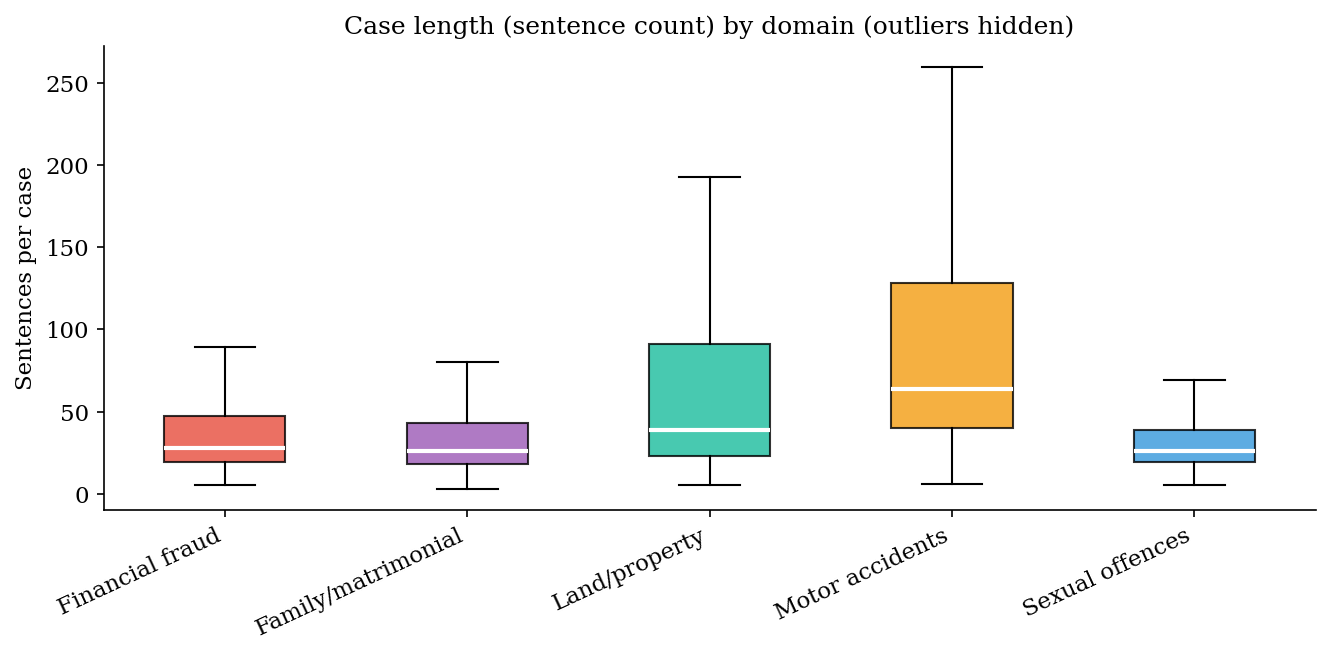
\includegraphics[width=0.92\textwidth]{figures/06_sentence_count_distribution_full.png}
  \caption{Sentence-count distribution per legal domain bucket across the full
  corpus. Land-property and financial-fraud have the heaviest right tails (long,
  document-heavy judgments); motor-accidents is concentrated at low sentence
  counts (short tribunal orders). These distributions directly drove the per-bucket
  chunking strategy for \texttt{bge-m3} embedding.}
  \label{fig:sentence_count_dist}
\end{figure}

The distributions confirm the ordering expected from domain knowledge.
Motor-accidents judgments are typically short and tribunal-style, concentrated
well below 100 sentences. Land-property matters are long and document-heavy
(deeds, surveys, possession history), with a pronounced right tail extending into
several hundred sentences per case. Financial-fraud and family-matrimonial sit
between these extremes. Sentence-count distributions follow the same ordering as
overall document length and are the primary driver of the hierarchical-chunking
configuration in Section~\ref{sec:text_features}: long-tail \textsc{Facts} and
\textsc{Arguments} sections in land-property and financial-fraud buckets exceed
the \texttt{bge-m3} context window and are mean-pooled across overlapping chunks,
with the chunk boundary set per-bucket based on the 90th-percentile sentence
count.

\subsection{Entity Richness Per Domain}

Entity richness --- the number of unique canonicalised entities per case --- is
a per-domain structural property that predicts both graph density and expected
modelling difficulty. A domain where every case cites a wide variety of distinct
statutes, provisions, and precedents will produce a denser, more richly
interconnected subgraph; a domain where cases repeatedly cite the same small set
of authorities will produce a sparser subgraph with lower information diversity
per case. Figure~\ref{fig:richness_and_degree} plots entity richness alongside
mean case degree for each bucket, providing a direct comparison of both
dimensions.

\begin{figure}[H]
  \centering
  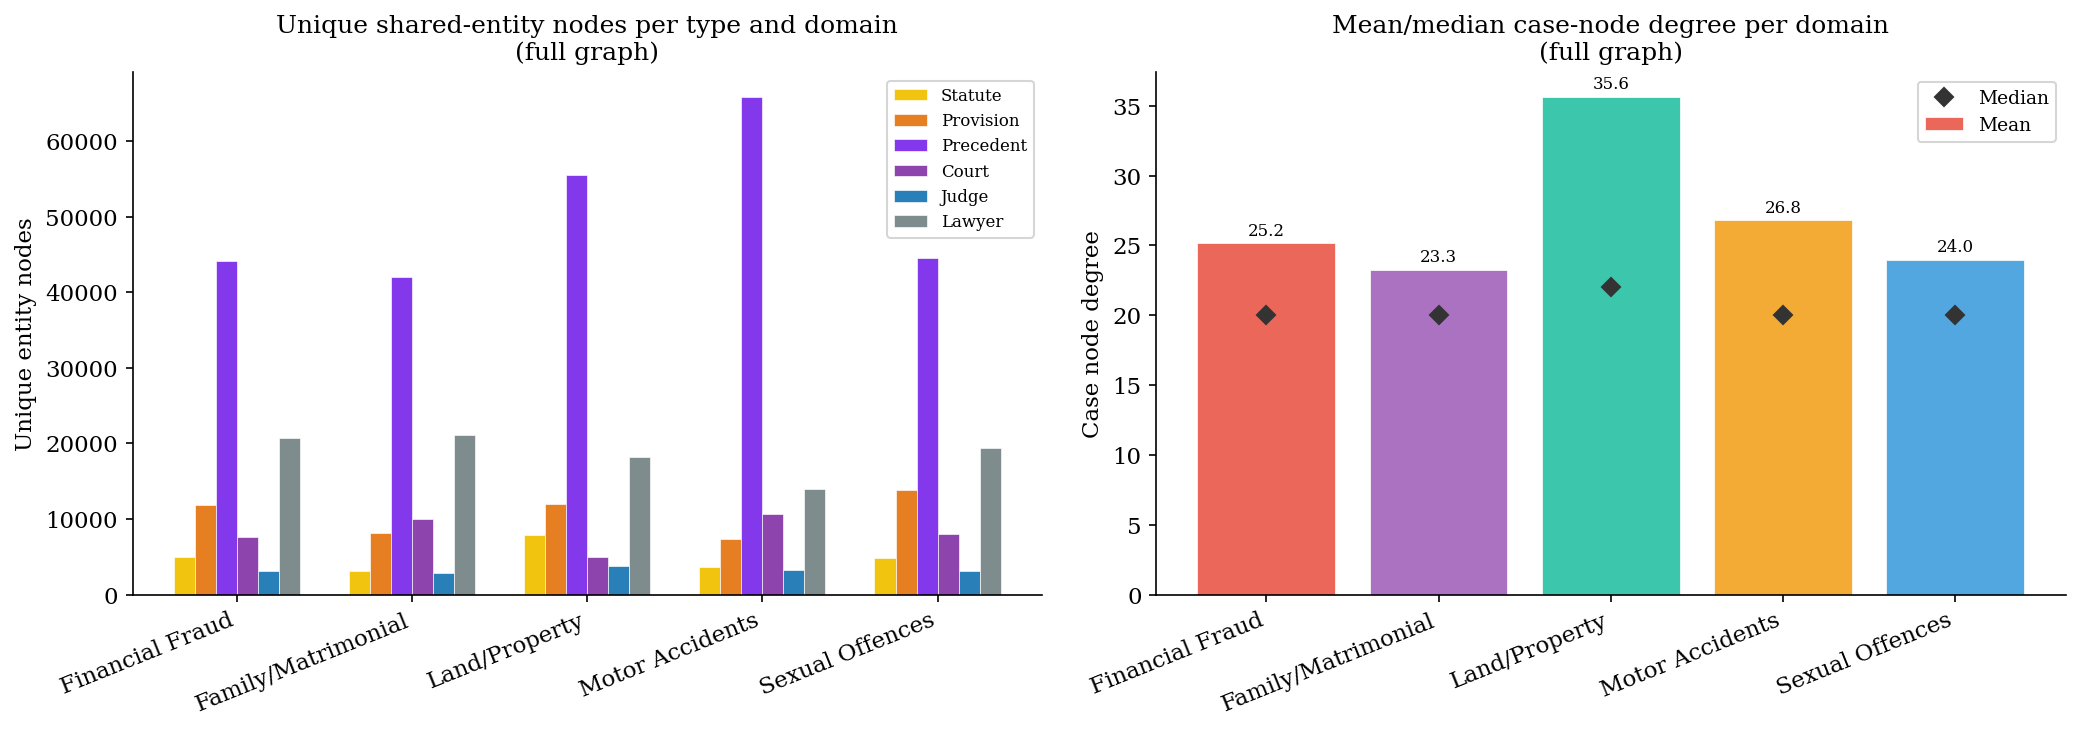
\includegraphics[width=0.92\textwidth]{figures/38_per_bucket_richness_and_degree.png}
  \caption{Entity richness (unique canonicalised entities per case) and mean case
  degree per legal domain bucket. Land-property and financial-fraud are both
  entity-rich and highly connected; motor-accidents is entity-poor and
  low-degree. The correlation between richness and degree confirms that these
  are domain-level phenomena rather than noise effects.}
  \label{fig:richness_and_degree}
\end{figure}

The figure confirms the expected ordering. Land-property and financial-fraud
score highest on both axes: their cases cite many distinct statutes, provisions,
and precedents, and are therefore well-connected to the graph's shared-entity
layer. Motor-accidents scores lowest on both: it repeatedly cites the same narrow
provision set (\textsc{Motor Vehicles Act~1988}, Section~166) and produces cases
with comparatively few graph edges. The correlation between richness and degree is
expected --- a case that cites many distinct authorities will naturally have more
edges --- but the per-domain consistency confirms that this is a domain-level
structural phenomenon rather than variance driven by outlier cases. Domains with
high richness and degree will benefit more from multi-hop message passing than
sparse domains; the ablation in Chapter~\ref{chap:results} tests this prediction
directly.

The PageRank ranking within each bucket makes the domain fingerprint concrete:

\begin{itemize}
  \item \textbf{Family \& Matrimonial}: IPC, CrPC, Sections~498A, 482.
  \item \textbf{Financial Fraud}: IPC, CrPC, Sections~420, 468, 471.
  \item \textbf{Land \& Property}: Supreme Court, Land Acquisition
    Act~1894, Constitution of India.
  \item \textbf{Motor Accidents}: Motor Vehicles Act~1988, Supreme Court,
    Apex Court, Section~166.
  \item \textbf{Sexual Offences}: IPC, CrPC, POCSO Act, Section~506.
\end{itemize}

The top-5 per bucket is a near-perfect fingerprint of the underlying
legal domain, which is a reassuring sanity check: the canonicalisation
and the NER are recovering legally meaningful primary citations, not
surface noise.

The table above tells us \emph{which} entities are important; it does not tell
us \emph{how} they are organised relative to each other within the bucket.
A domain where the top-ranked entities form a tight, star-shaped cluster around
a single authority behaves very differently from one where the top entities form
a distributed, multi-centred network --- even if the ranked lists look superficially
similar. Figure~\ref{fig:within_bucket_network_fingerprints} makes this geometry
visible by showing the entity co-occurrence network within each bucket restricted
to its top-25 PageRank entities. This is the strongest diagnostic available for
whether the domain fingerprints recovered by canonicalisation are structurally
coherent, not just statistically high-ranking.

\begin{figure}[H]
  \centering
  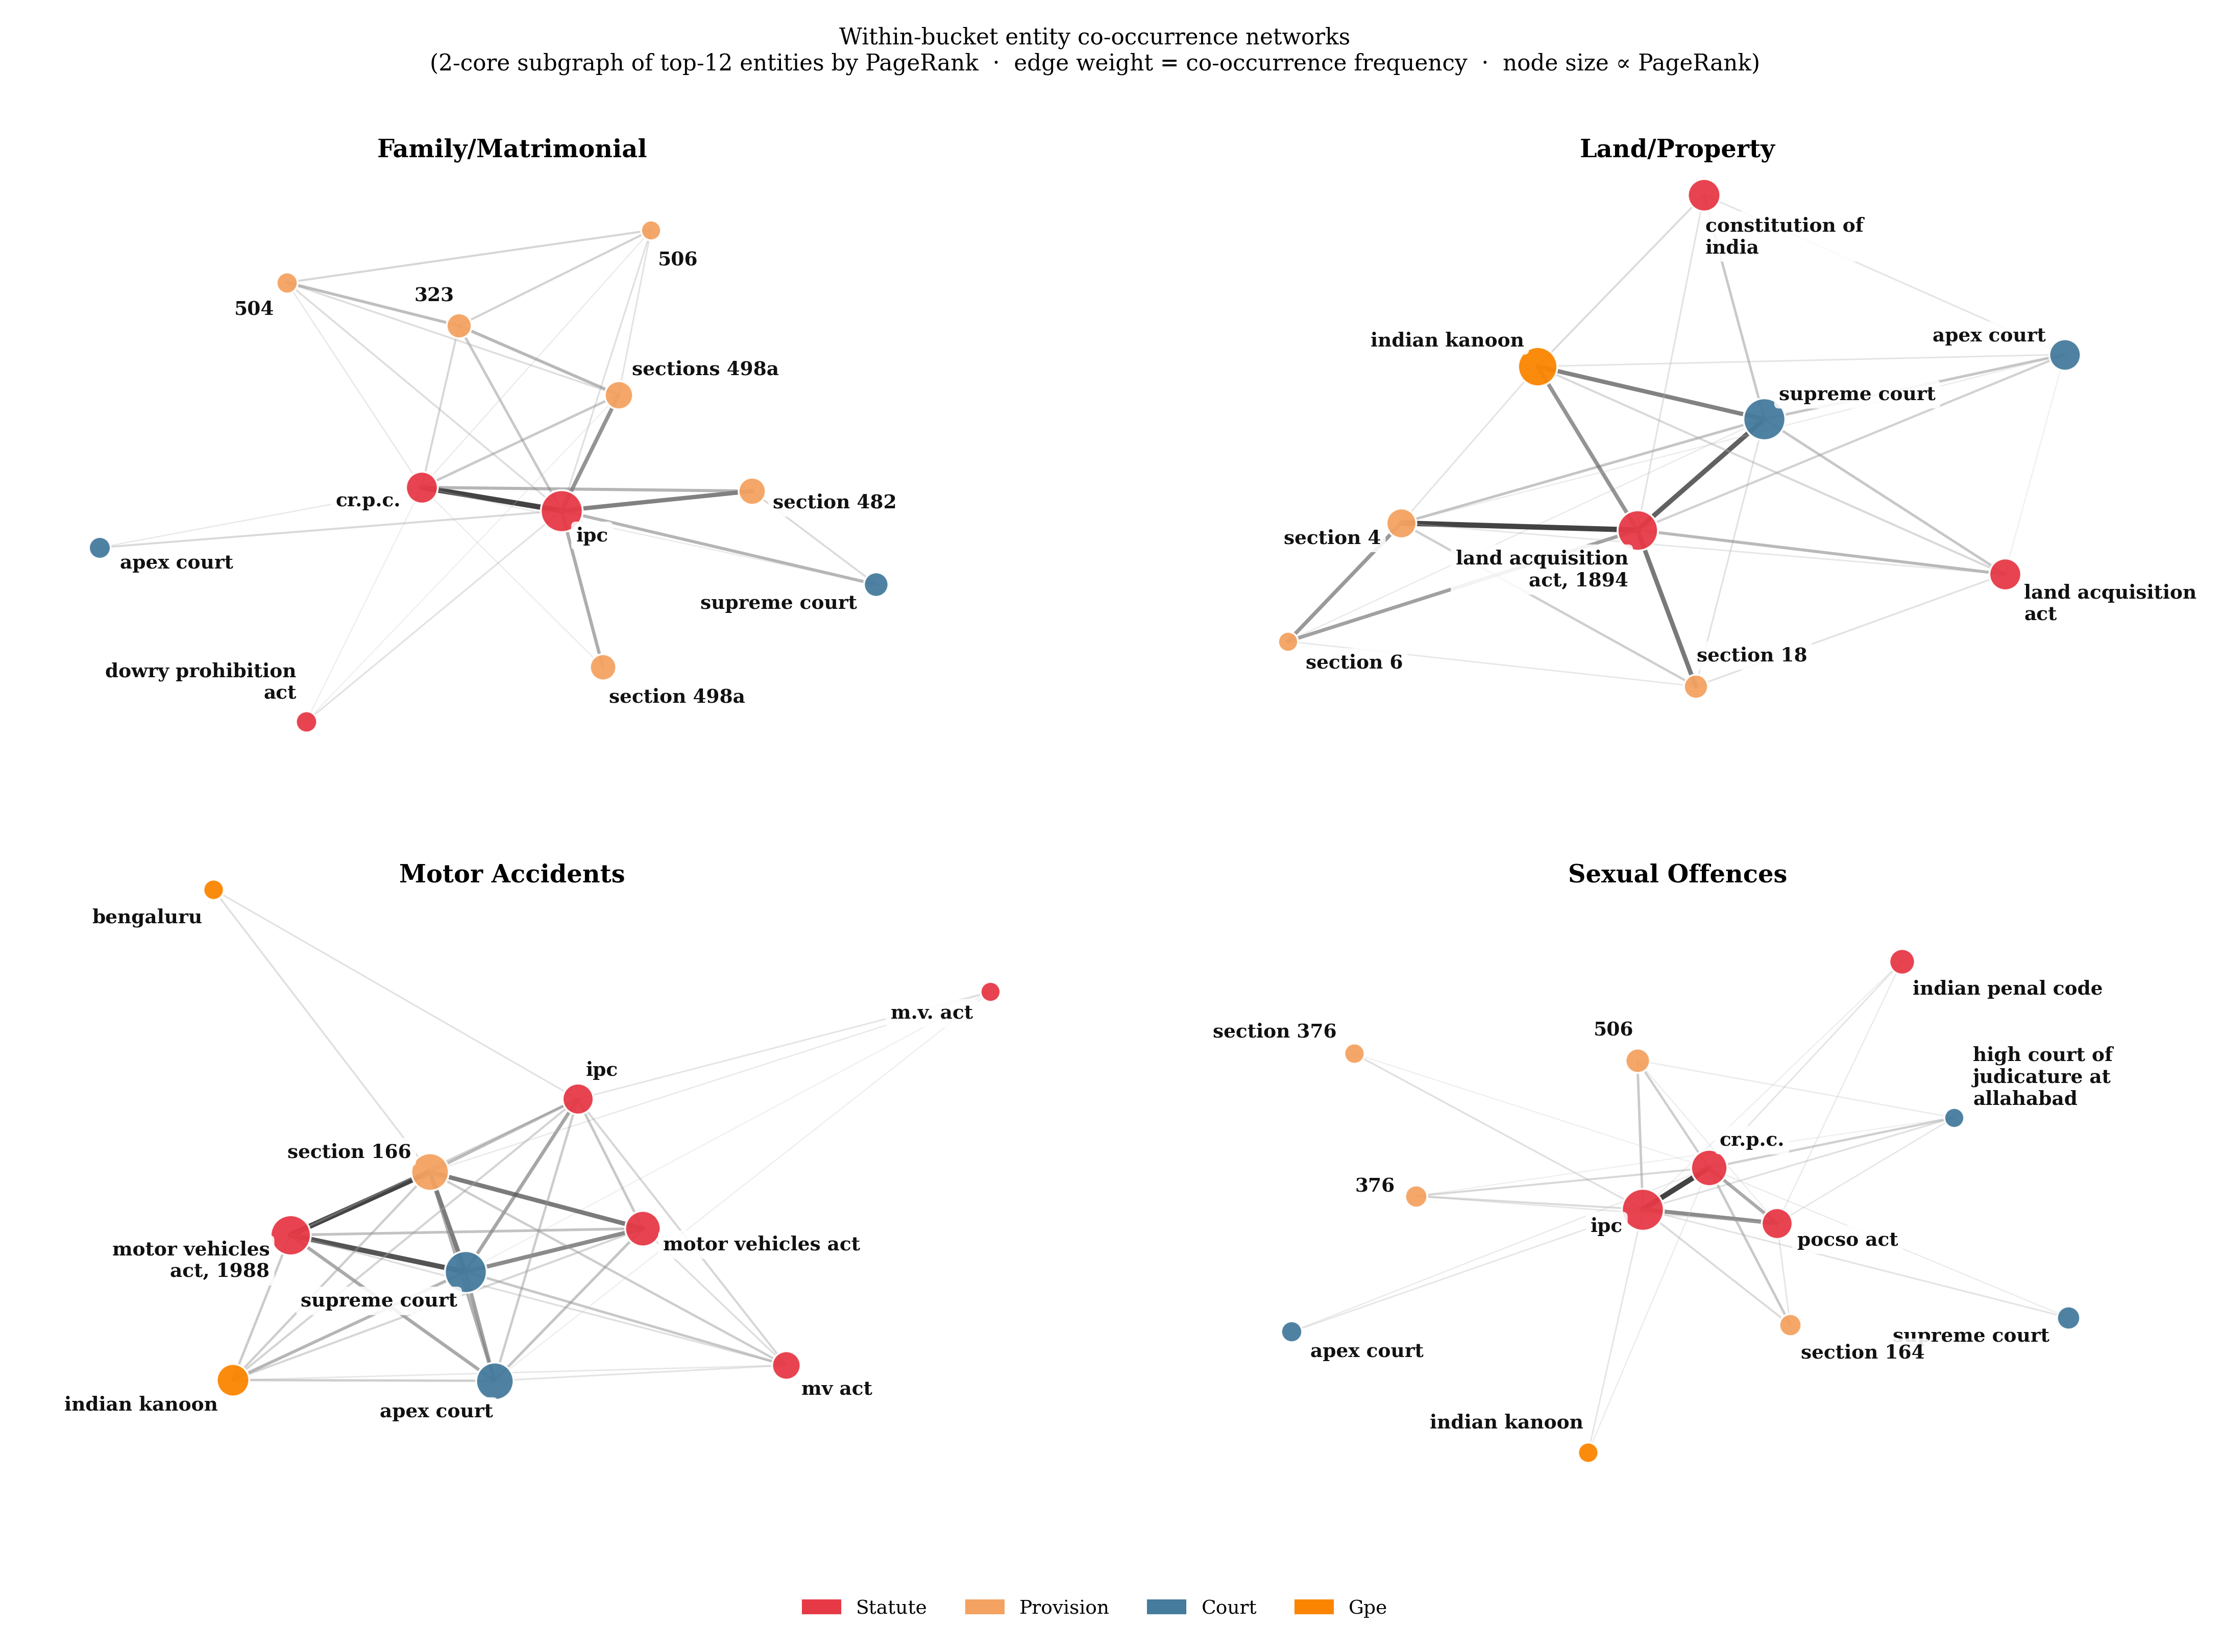
\includegraphics[width=\textwidth]{figures/36_within_bucket_network_fingerprints.png}
  \caption{Within-bucket entity co-occurrence networks for four legal domains,
  each restricted to the top-25 PageRank entities in that bucket. Node size is
  proportional to PageRank score. The figure reveals not just which entities rank
  highest but how they are geometrically organised: tight criminal-procedure stars
  in family-matrimonial and sexual-offences, a distributed multi-centred structure
  in land-property, and an extremely compact low-diversity backbone in
  motor-accidents.}
  \label{fig:within_bucket_network_fingerprints}
\end{figure}

The networks reveal that the domains differ not only in their top entities but in
their \emph{network geometry}, and that the differences are legally interpretable.
Family~\&~matrimonial and sexual offences both remain visibly
\textsc{IPC}/\textsc{CrPC}-centred, yet they bifurcate into distinct provision
clusters almost immediately below the top hub: Section~498A, 482, and
dowry-related citations form the inner ring in family-matrimonial, while
\textsc{POCSO}, Section~376, and Section~363 dominate in sexual offences. The
two domains share the same criminal-procedure spine but are routed through
different specialised provisions — exactly the relationship predicted by the
entity-sharing matrix (Figure~\ref{fig:cross_bucket_sharing_matrix}).

Land-property is geometrically distinct from both: its network is spatially
spread with several semi-central statutory and constitutional nodes rather than
one overwhelmingly dominant criminal-procedure core. The \textsc{Land Acquisition
Act~1894} and the \textsc{Constitution of India} sit as co-equal secondary hubs
alongside \textsc{Supreme Court}, forming a multi-centred structure that reflects
the domain's diverse statutory and constitutional basis and is consistent with
its higher entity richness shown in Figure~\ref{fig:richness_and_degree}.

Motor-accidents, by contrast, exhibits the tightest and most repetitive local
backbone of all four domains, with \textsc{Motor Vehicles Act~1988} and
Section~166 forming an extremely compact star. The near-absence of peripheral
nodes confirms that most motor-accidents cases enter the graph through the same
narrow set of recurring authorities, leaving little structural diversity for
multi-hop message passing to exploit. This visual finding is the network-geometry
counterpart of the low connectivity score and low entity richness established in
the preceding subsections.

Together, these bucket-level network snapshots make the domain-fingerprint claim
visual rather than purely tabular, and provide structural grounding for the
prediction chapter: domains with richer, more spread network geometry (land-property,
financial-fraud) can be expected to benefit more from multi-hop message passing
than domains with tight, low-diversity backbones (motor-accidents).

The within-bucket view, however, treats each domain in isolation. To understand
how entities are \emph{shared} or \emph{segregated} across all five domains
simultaneously, Figure~\ref{fig:cross_domain_network_fingerprint} collapses the
five independent networks into a single cross-domain graph. Each domain is
represented as a large hub node placed at the vertex of a pentagon; the top-10
PageRank entities from each domain appear as satellite nodes, connected to
whichever hubs they belong to. Entities that appear in the top-10 of two or more
domains are drawn with a bold outline and linked by crimson cross-domain edges,
making the inter-domain bridges immediately legible.

\begin{figure}[H]
  \centering
  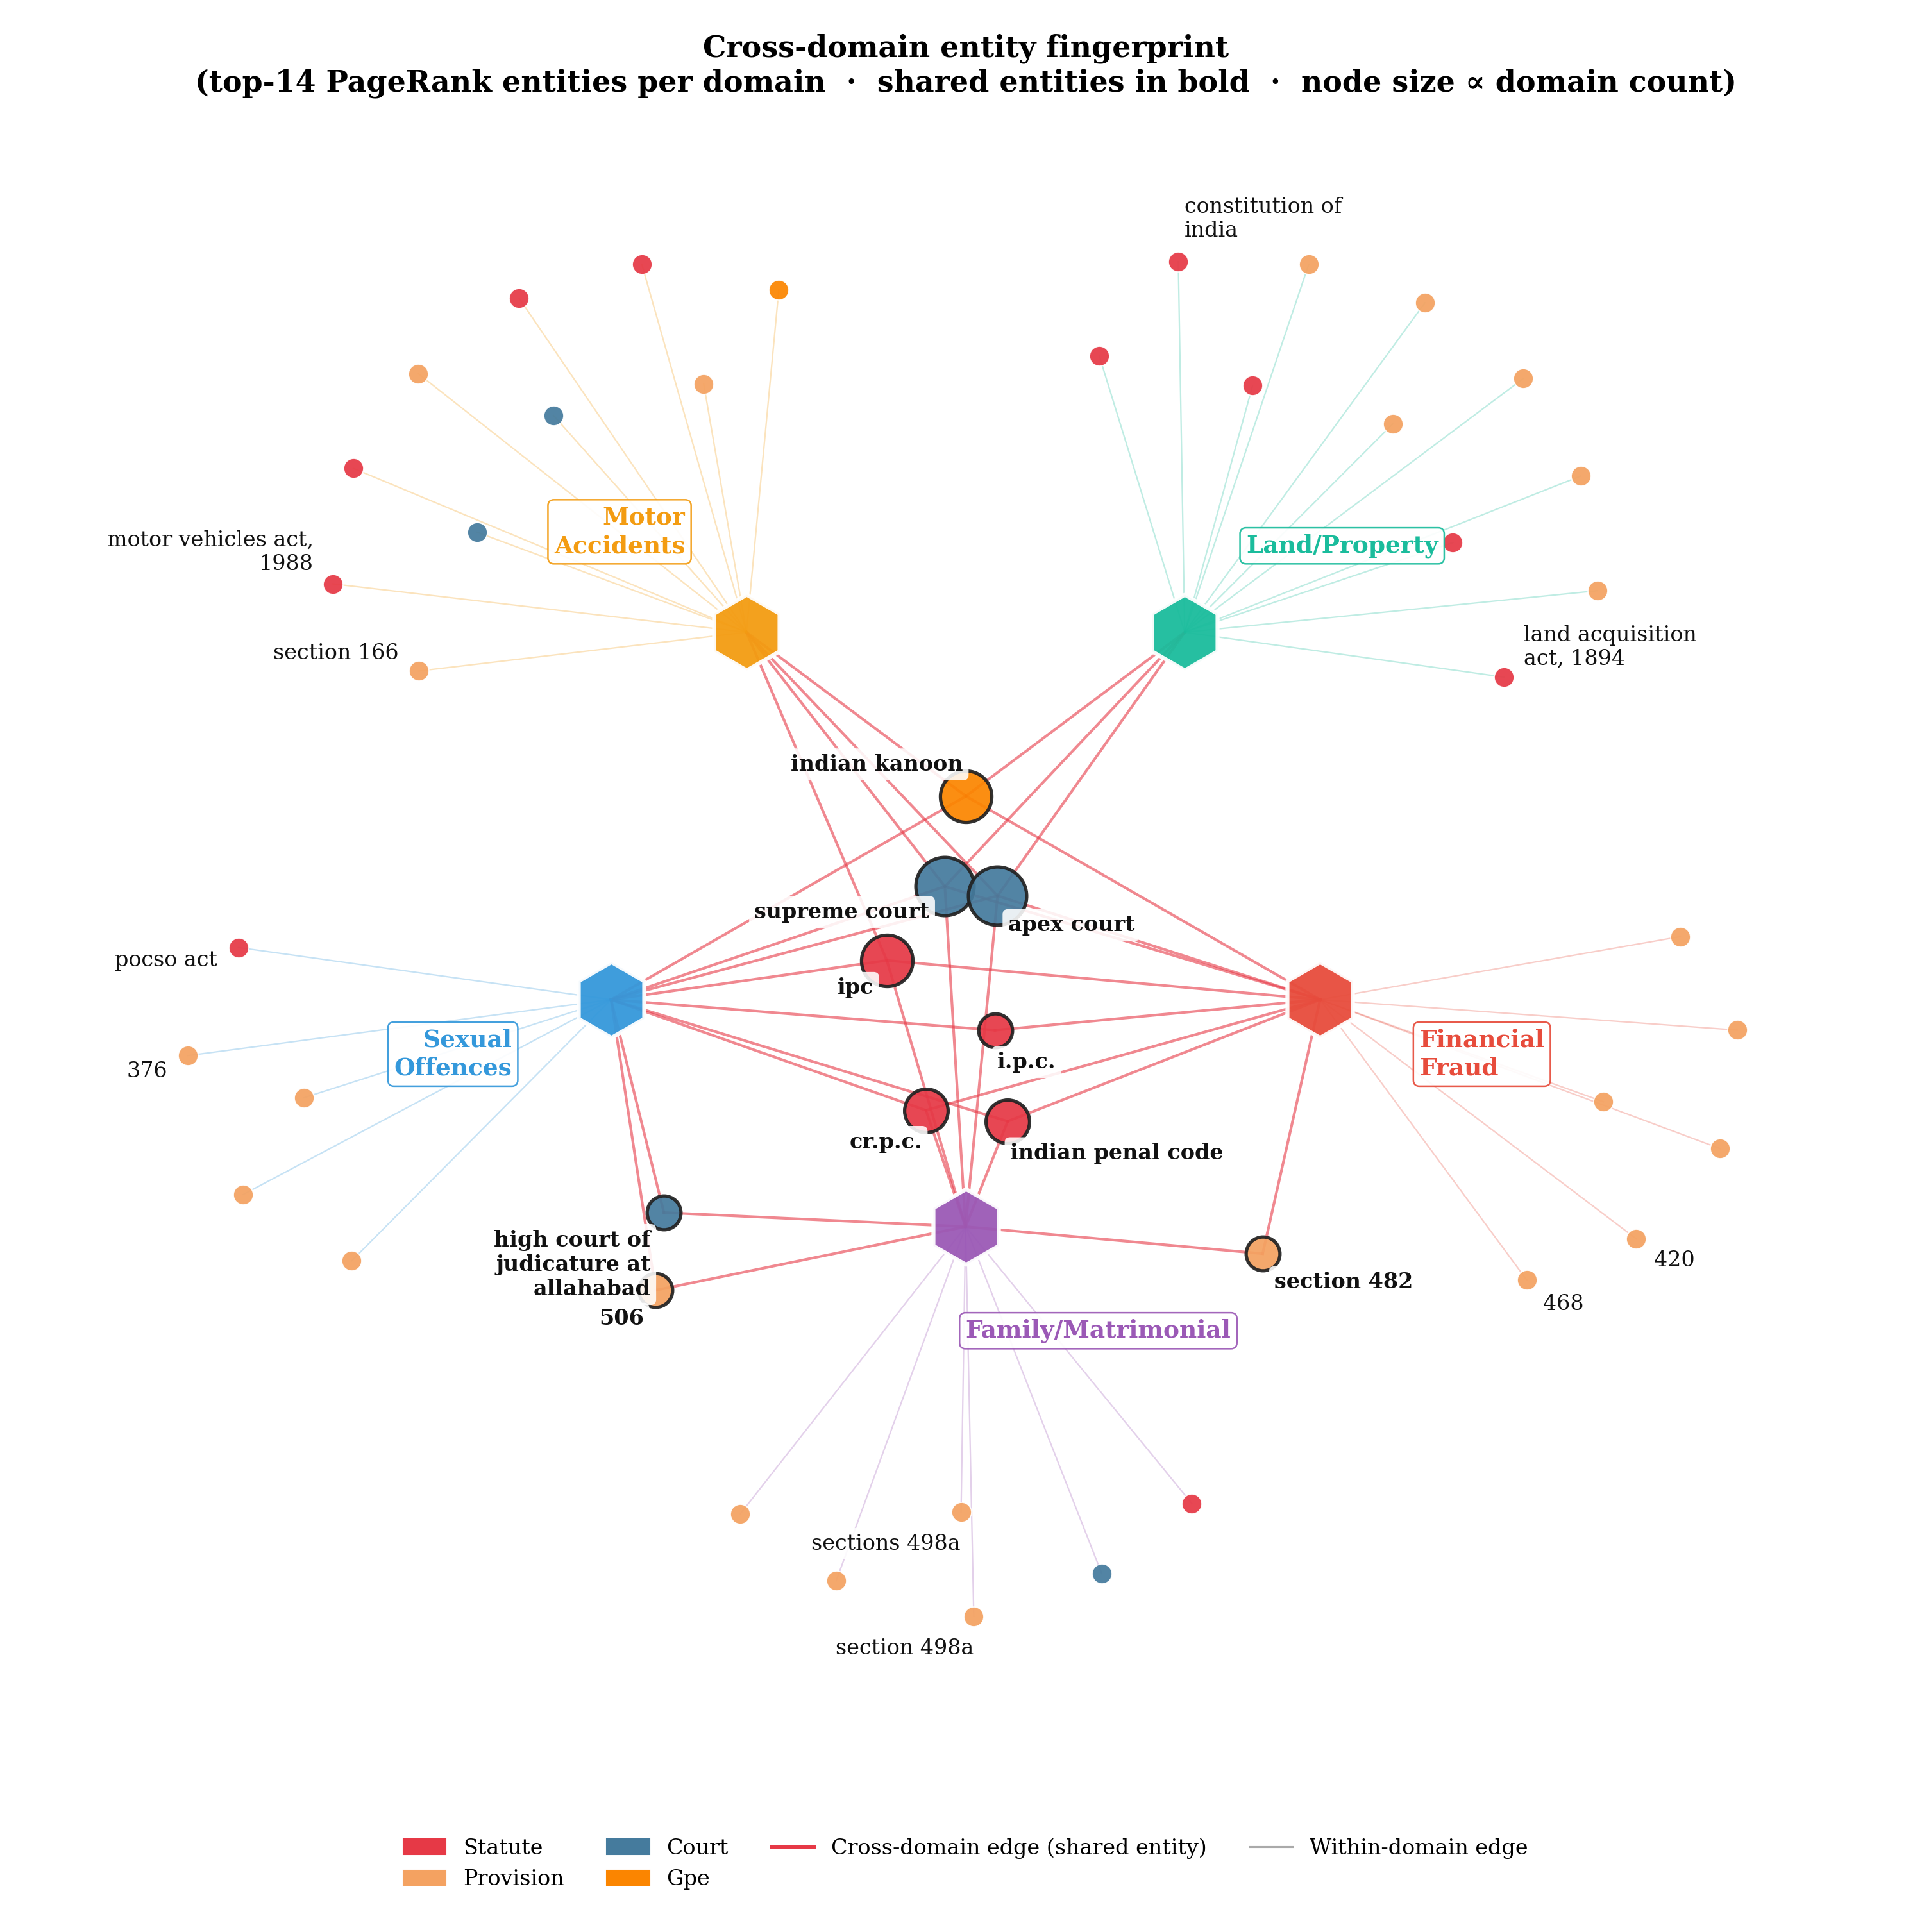
\includegraphics[width=\textwidth]{figures/44_cross_domain_network_fingerprint.png}
  \caption{Cross-domain entity fingerprint: the top-10 PageRank entities from
  each of the five legal domains are placed around five domain-hub nodes arranged
  in a pentagon. Node colour encodes entity type; node size encodes the number of
  domains the entity appears in. Crimson edges connect entities that bridge two or
  more domains; domain-coloured edges connect exclusive entities to their single hub.}
  \label{fig:cross_domain_network_fingerprint}
\end{figure}

The cross-domain view reveals a clear three-tier bridge structure. At the widest
tier, \textsc{Supreme Court} and \textsc{Apex Court} appear in the top-10 of all
five domains — universal procedural anchors that carry interpretive weight
regardless of substantive legal area. At the intermediate tier, \textsc{IPC},
\textsc{CrPC}, and \textsc{Section~482} bridge the three criminal-procedure
domains (Family/Matrimonial, Financial Fraud, and Sexual Offences) but are absent
from the top tier of Land/Property and Motor Accidents — confirming that the
criminal-procedure spine is real but domain-bounded. At the narrowest tier,
domain-exclusive entities (\textsc{Land Acquisition Act~1894} for land-property,
\textsc{Motor Vehicles Act~1988} and \textsc{Section~166} for motor-accidents,
\textsc{POCSO} for sexual offences) remain firmly segregated, appearing only in
the satellite cluster of their single hub. This stratified bridge structure is
precisely what a well-designed heterogeneous graph should exhibit: enough shared
structure for cross-domain representation learning, but enough domain exclusivity
for the GNN to recover meaningful per-domain fingerprints rather than collapsing
all five into a single undifferentiated embedding.

\subsection{Rhetorical Role Composition Per Domain}

The rhetorical-role composition of the training corpus matters for two reasons.
First, \textsc{RPC} and \textsc{RLC} annotations are the primary leakage vector
and must be absent from the cleaned graph; verifying their absence domain by
domain is a structural safety check, not just a logical one. Second, the relative
sizes of the remaining blocks (\textsc{Facts}, \textsc{Arguments},
\textsc{Preamble}) determine the text-feature distribution the GNN trains on, and
domain differences in those proportions explain part of the per-domain variation
in embedding quality. Figure~\ref{fig:rr_breakdown} shows the rhetorical role
breakdown after leakage-safe filtering.

\begin{figure}[H]
  \centering
  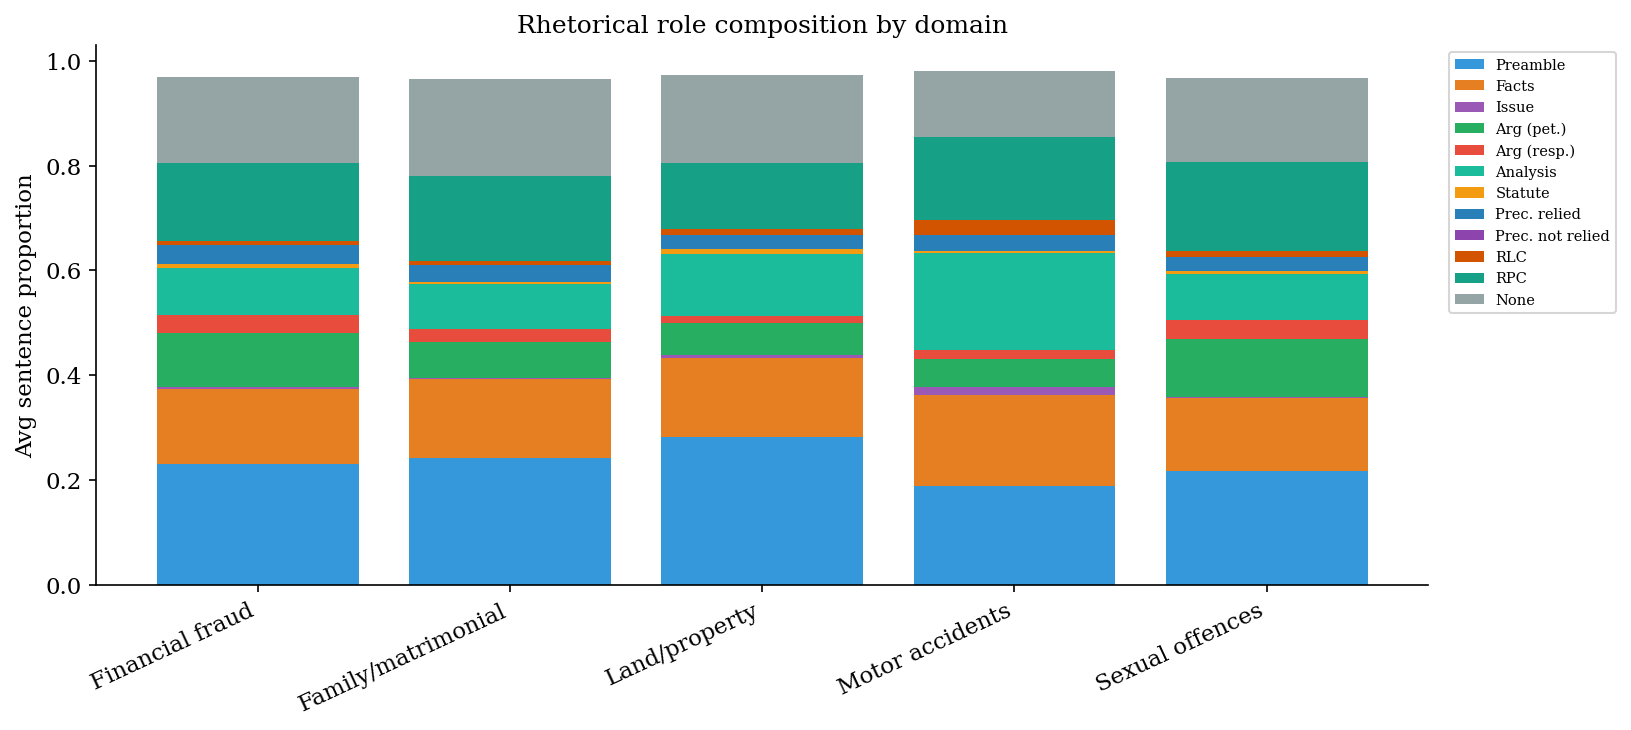
\includegraphics[width=0.95\textwidth]{figures/07_rhetorical_role_breakdown_full.png}
  \caption{Rhetorical role breakdown per bucket after leakage-safe filtering.
  \textsc{RPC} and \textsc{RLC} annotations are intentionally absent, confirming
  the leakage gate is effective across all five domains. \textsc{Facts} and
  \textsc{Arguments} dominate; the relative size of \textsc{Arguments} tracks
  case length, being largest in land-property and financial-fraud.}
  \label{fig:rr_breakdown}
\end{figure}

The composition after filtering is dominated by \textsc{Facts} and
\textsc{Arguments}, with a stable \textsc{Preamble} share across domains. The
relative size of the \textsc{Arguments} block tracks case length: it is largest
in land-property and financial-fraud and smallest in motor-accidents, consistent
with the sentence-count distributions in Section~\ref{sec:perdomain}. The
complete absence of \textsc{RPC} and \textsc{RLC} labels confirms that the
leakage filter is operating correctly across all five buckets.

\subsection{Outcome Distribution Per Domain}

The outcome label distribution and its per-domain win/loss rates were analysed
in detail as part of the pipeline audit in
Chapter~\ref{chap:pipeline} (Figures~\ref{fig:outcome_distribution}
and~\ref{fig:outcome_rate}). From the graph-exploration perspective, the relevant
structural observation is that the class imbalance is \emph{domain-dependent}:
motor-accidents is the most win-skewed, financial-fraud and sexual-offences sit
closest to balanced. This means the GNN's training signal is not uniformly
imbalanced --- different domains present different prior odds --- which in turn
means that per-domain calibration, rather than a single global threshold,
is the appropriate evaluation design. The cross-bucket pooled win rate of
roughly $60\%$ to $40\%$ is why Chapter~\ref{chap:results} reports macro-F1
alongside accuracy and ROC-AUC as co-primary metrics.

\section{Key Structural Insights}
\label{sec:key_insights}

Five insights carry forward into the prediction chapter:

\begin{enumerate}
  \item \textbf{The graph is hub-dominated.} A small number of
    cross-bucket statutes and courts (IPC, CrPC, Supreme Court) are
    the spine of the graph; most other entities are long-tail leaves.
    Any claim the model makes about ``cross-case reasoning'' must be
    interpretable against this topology.
  \item \textbf{Cross-domain sharing is real but uneven.} The four
    IPC/CrPC-driven buckets share heavily with each other; land-property
    partially detaches via its own statutory backbone. A cross-domain
    model should outperform a naive concatenation only if it can
    actually exploit the shared spine.
  \item \textbf{Identity-proxy leakage is structural.} Judges,
    specific lawyers, and specific courts have bridge and betweenness
    scores high enough to make \emph{sharing} them across cases
    unsafe; the decision to hold them local is vindicated by the
    bridge analysis.
  \item \textbf{Connectivity score predicts modelling difficulty.}
    Low-connectivity cases have, by construction, fewer shared-entity
    neighbours to aggregate from; the per-domain accuracy pattern in
    Chapter~\ref{chap:results} is consistent with connectivity being a
    first-order driver of case-level difficulty.
  \item \textbf{The per-domain fingerprints are legally coherent.}
    Each bucket's top-PageRank entities are exactly what a lawyer
    would expect; this is the single strongest evidence that the
    pipeline's NER, canonicalisation, and rhetorical-role filtering
    together produce a legally faithful, not merely statistically
    clean, corpus.
\end{enumerate}
